\section{绪论}

\begin{frame}{绪论}
    \begin{columns}
        \begin{column}{0.5\textwidth}
        \includegraphics[scale=0.3]{figures/smartcity.jpg}
        \end{column}

        \begin{column}{0.5\textwidth}
        \textbf{智慧城市:} 
        
        数字城市、物联网、云计算
        \vspace{2em}

        \pause
        \alert{数字城市}
        \begin{itemize}
        \item 空间信息快速获取技术
        \item 海量空间数据管理技术
        \item 空间信息可视化技术
        \item 空间数据分析挖掘技术
        \item $\ldots$
        \end{itemize}
        \end{column}
   \end{columns}
\end{frame}

\begin{frame}{绪论}
    \textbf{移动互联网发展}

    \alert{LBS应用}
    打车软件、O2O软件、社交网络软件

    \vspace{2em}
    \pause
    \textbf{意义}
    \begin{itemize}
        \pause
        \item 对个人而言(智慧生活)
        \pause
        \item 对商业公司而言(智慧商业)
        \pause
        \item 对政府决策部门而言(智慧政府)
    \end{itemize}
\end{frame}

\begin{frame}[t]{绪论}
% \alert{海量数据处理}

% 业界使用Hadoop并行计算框架,但是存在处理速度慢、计算抽象层次较低等缺陷。

% \pause
% Spark是新型的并行计算框架,内存计算速度快,算子表现力丰富。但是对空间数据类型和空间数据操作支持不够。

\begin{columns}
    \begin{column}{0.4 \textwidth}

        \begin{center}
        \alert{海量数据处理}

        \vspace{1em}
        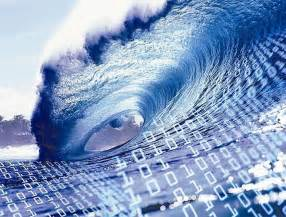
\includegraphics[height=3.5cm]{figures/seaamountdata.jpeg}
        \end{center}


    \end{column}

    \pause
    \begin{column}{0.6 \textwidth}

        \begin{center}
            \alert{并行计算}

            \vspace{1em}
            \includegraphics[height=3.5cm]{figures/parallelcomputation.png}
        \end{center}
       
    \end{column}

\end{columns}

% \vspace{2em}

% \pause
% \alert{并行化算法设计}

% 空间数据挖掘算法并没有针对并行化计算框架进行设计。

\end{frame}

\begin{frame}[c]{绪论}
    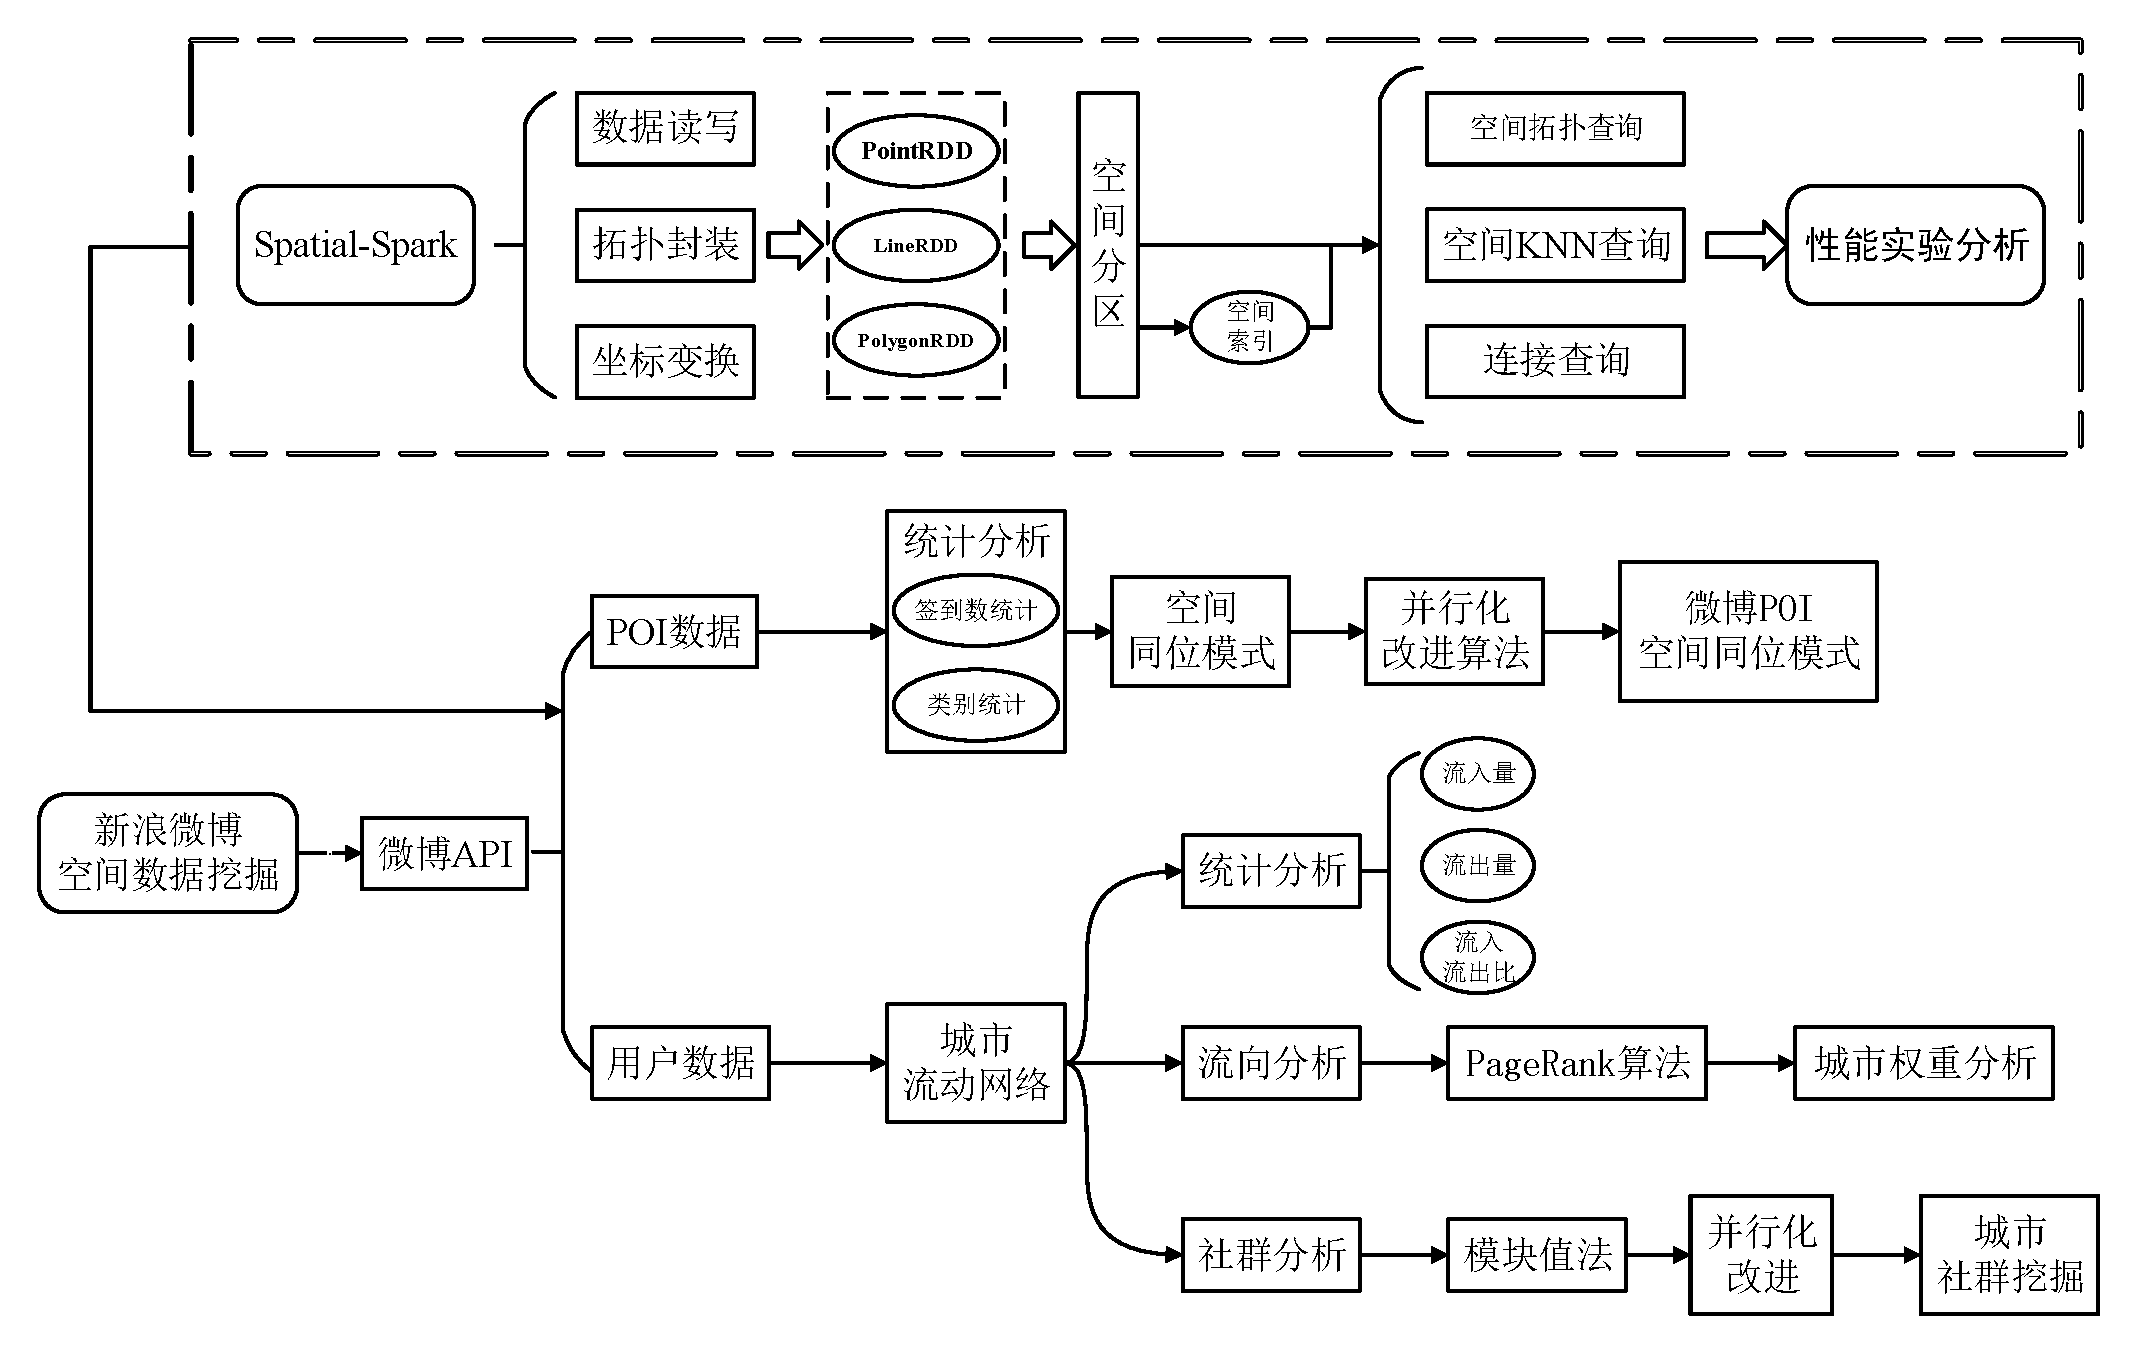
\includegraphics[scale=0.3]{figures/technology_route.pdf}
\end{frame}